\exam{2024}
\begin{problem}{Poisson Process}
Suppose we construct an arrival process from a Poisson process by shifting each arrival by $\Delta_i$ to the right with probability $p_i$, for $i = 1, \ldots, 10$. Why is the constructed arrival process a Poisson process from time $t = \max_i \Delta_i$ onwards?
\end{problem}

\begin{problem}{Discrete-Time Markov Chains}
Give an example of a Markov chain where all the states have period 2 with at least one transient state and at least one recurrent state.
\end{problem}

\begin{solution}
  \begin{figure}[h!]
    \begin{center}
      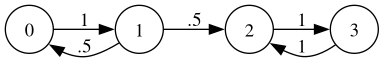
\includegraphics[width=0.5\textwidth]{img/24.2.png}
    \end{center}
  \end{figure}
\end{solution}

\begin{problem}{Discrete-Time Markov Chains}
Consider a single roll of 5 dice. Set up a DTMC that allows you to compute the probability of having a full house, meaning the result of the roll is three dice with one number and two dice with another number (5 identical numbers do not count). Try to minimize the number of states in your DTMC. There is no need to compute the actual probability.
\end{problem}
\begin{problem}{Discrete-Time Markov Chains}
  Let $(X_n)_{n\geq 0}$ be an irreducible aperiodic DTMC. Let the $(Y_n)_{n\geq0}$ be the DTMC obtained by censoring out state 0 of $(X_n)_{n\geq 0}$. In other words the DTMC $(Y_n)_{n\geq0}$ is identical to $(X_n)_{n\geq0}$ except that the points in time where state 0 is visited are skipped. Is $(Y_n)_{n\geq0}$ necessarily aperiodic? Prove this or give a counter example.
\end{problem}
\begin{solution}
  When removing state 0, we find a periodic DTMC.

  \begin{figure}[h!]
    \begin{center}
      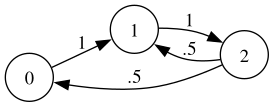
\includegraphics[width=0.3\textwidth]{img/24.4.png}
    \end{center}
  \end{figure}

\end{solution}

\begin{problem}{Continuous-Time Markov Chains}
Give an example of a positive recurrent CTMC $(X_t)_{t\geq 0}$ with an infinite number of states such that $\lim_{i\rightarrow\infty} D_i = 0$, where $D_i$ is the drift of the embedded Markov chain $(Y_n)_{n\geq 0}$ in state $i$, that is, $D_i = E[Y_{n+1} - Y_n|Y_n = i]$.
\end{problem}

\begin{problem}{Applications}
Consider an M/M/C queue. Suppose we increase the arrival rate and the rate of each of the $C$ servers by a factor $k$. Does this affect the queue length distribution? Explain. What about the mean response time? [Hint: You can answer this last question using a simple formula].
\end{problem}
\begin{solution}
The queue length distribution in an M/M/C system depends on the traffic intensity $\rho = \frac{\lambda}{C\mu}$. If both the arrival rate $\lambda$ and the service rate $\mu$ are scaled by a factor $k$, the new traffic intensity becomes:

\[
\rho' = \frac{k\lambda}{C \cdot k\mu} = \rho.
\]

Since $\rho$ remains unchanged, the queue length distribution is unaffected.

For the mean response time $W$, which can be expressed as the sum of the mean waiting time in the queue and the mean service time:

\[
W = W_q + \frac{1}{\mu},
\]

scaling $\mu$ by a factor $k$ reduces the mean service time to $\frac{1}{k\mu}$. Therefore, while the waiting time $W_q$ remains unchanged (as it depends on $\rho$), the mean response time decreases.

Intuitively, this result makes sense: the system processes jobs faster due to the higher service rate, but the balance of arrivals and departures remains the same, preserving the queue's overall behavior.
\end{solution}

\begin{problem}{Applications}
  Consider a Jackson network in which each of the $M$ queues is replaced by an infinite number of servers, where the speed of a single server is $\mu_i$ for queue $i$. Assume the routing is such that $(I - P )^{-1}$ exists. Consider the CTMC that keeps track of the number of busy servers in each queue. Derive the global balance equations for this CTMC. Clearly explain the different terms appearing in your equations. What is the condition needed for the Markov chain to be positive recurrent? Give an expression for the stationary distribution (without actually proving it)
\end{problem}
\begin{solution}
    We can write the global balance equation as
    \begin{align*}
    \lambda_0 \pi(\mathbf{n})
    + \sum_{i=1}^M p_{i0} \pi(\mathbf{n}) \mu_i n_i 1[n_i > 0]
    &= \sum_{i=1}^M \lambda_0 p_{0i} \pi(\mathbf{n} - \mathbf{e}_i) \\
    &\quad + \sum_{i=1}^M \mu_i n_i p_{i0} \pi(\mathbf{n} + \mathbf{e}_i) \\
    &\quad + \sum_{\substack{i,j=1 \\ i \neq j}}^M \mu_j n_j p_{ji} \pi(\mathbf{n} + \mathbf{e}_j - \mathbf{e}_i).
    \end{align*}

    \begin{itemize}
        \item $\lambda_0 \pi(\mathbf{n})$: \\
            Represents the rate at which external arrivals contribute to the state $\mathbf{n}$.
        \item $\sum_{i=1}^M p_{i0} \pi(\mathbf{n}) \mu_i n_i 1[n_i > 0]$: \\
            Accounts for the departures from the system to an external sink, where a job leaves the queue at rate $\mu_in_i$ given there is at least one job in queue $i$.
        \item $\sum_{i=1}^M \lambda_0 p_{0i} \pi(\mathbf{n} - \mathbf{e}_i)$: \\
            This term represents external arrivals into queue $i$.
        \item $\sum_{i=1}^M \mu_i n_i p_{i0} \pi(\mathbf{n} + \mathbf{e}_i)$: \\
            This term represents jobs leaving the system entirely.
        \item $\sum_{\substack{i,j=1 \\ i \neq j}}^M \mu_j n_j p_{ji} \pi(\mathbf{n} + \mathbf{e}_j - \mathbf{e}_i)$: \\
            This term represents jobs moving between queues.
    \end{itemize}

    The routing matrix $P$ satisfies $(I - P )^{-1}$, ensuring a stable flow in the network. As long as $\lambda_i$ is finite and $\mu_i > 0$, the CTMC is positive recurrent.

    The stationary distribution can be described as
    \[
        \pi(\mathbf{n}) = \prod_{i=1}^M\frac{\rho_i^{n_i}}{n_i!}\exp(-\rho_i)
    \]

    \textbf{Note}: The whole excercise is a variant on Jackson's theorem.
\end{solution}
